\documentclass{weeklyprogress}

\title{Progress Report: Week 0}
\author{Jingyi Long}

\begin{document}

\section{Theoretical Bounds for Finding Integer Relations}

\begin{definition}[Integer relation problem]
Let $\bm{a}_1,\ldots,\bm{a}_m\in\mathbb{R}^n$ be vectors that are linearly dependent over $\mathbb{Q}$. Denote $A = \begin{bmatrix}\bm{a}_1 &\cdots &\bm{a_m}\end{bmatrix}$. An \emph{integer relation} among these vectors is a nonzero coefficient vector $\bm{x}=(x_1,\ldots,x_m)\in\mathbb{Z}^m$ such that
\[ A \bm{x} = \sum_{i=1}^m x_i\bm{a}_i=\bm{0}. \]
The integer relation problem is to find such a vector $\bm{x}$.
\end{definition}

The difficulty is that, because of numerical error and the finite precision of computer arithmetic, only approximations $\widetilde{\bm{a}}_1,\ldots,\widetilde{\bm{a}}_m$ are available. Suppose that $\lVert\widetilde{\bm{a}}_i-\bm{a}_i\rVert_\infty\leq\varepsilon$ for every $i$, and let $\bm{x}$ be a nontrivial integer relation having minimal $\lVert\bm{x}\rVert_\infty$. Then
\[ \left\lVert\sum_{i=1}^m x_i\widetilde{\bm{a}}_i\right\rVert_\infty=\left\lVert\sum_{i=1}^m x_i(\widetilde{\bm{a}}_i-\bm{a}_i)\right\rVert_\infty\leq\sum_{i=1}^m|x_i|\lVert\widetilde{\bm{a}}_i-\bm{a}_i\rVert_\infty\leq m\lVert\bm{x}\rVert_\infty\varepsilon. \]

To certify a relation from its numerical residual, nonrelations must produce residuals significantly larger than this error bound. The following proposition gives the scale on which small residuals can occur.

\begin{proposition}
Let $m,n,N\geq1$ be integers, and let $\bm{a}_1,\ldots,\bm{a}_m\in\mathbb{R}^n$ satisfy $\lVert\bm{a}_i\rVert_\infty<M$. There is a nonzero vector $\bm{x}\in\mathbb{Z}^m\cap[-N,N]^m$ such that
\[ \left\lVert\sum_{i=1}^m x_i\bm{a}_i\right\rVert_\infty<\frac{mMN}{\lfloor N^{m/n}\rfloor}\leq\frac{2mM}{N^{m/n-1}}. \]
\end{proposition}

\begin{proof}
For every $\bm{b}=(b_1,\ldots,b_m)\in\{0,\ldots,N\}^m$, consider the point $\sum_{i=1}^m b_i\bm{a}_i\in\mathbb{R}^n$. There are $(N+1)^m$ such points, and they lie in an axis-parallel box whose side lengths are all less than $mMN$. Set $q=\lfloor N^{m/n}\rfloor$ and partition each side of this box into $q$ intervals of equal length. This produces $q^n\leq N^m<(N+1)^m$ subboxes.

\begin{figure}[ht]
  \centering
  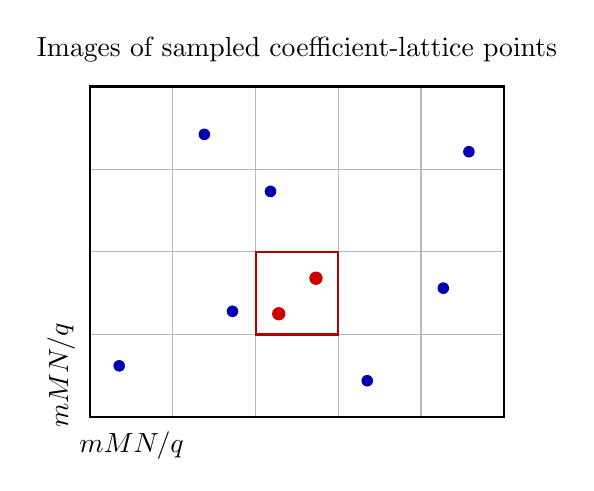
\begin{tikzpicture}[scale=1.05]
    \draw[step=1,gray!55,thin] (0,0) grid (5,4); \draw[thick] (0,0) rectangle (5,4); \foreach \p in {(0.35,0.62),(1.38,3.42),(1.72,1.28),(2.18,2.73),(3.35,0.44),(4.58,3.21),(4.27,1.56)} \fill[blue!70!black] \p circle (2pt); \fill[red!80!black] (2.28,1.25) circle (2.3pt); \fill[red!80!black] (2.73,1.68) circle (2.3pt); \draw[<->] (0,-0.35) -- node[fill=white,inner sep=1pt] {$mMN/q$} (1,-0.35); \draw[<->] (-0.35,0) -- node[fill=white,inner sep=1pt,rotate=90] {$mMN/q$} (-0.35,1); \draw[red!70!black,thick] (2,1) rectangle (3,2); \node[align=center] at (2.5,4.45) {Images of sampled coefficient-lattice points};
  \end{tikzpicture}
  \caption{Two-dimensional illustration of the subdivision. Each grid cell has side length less than $mMN/q$. The two red points occupy the same cell.}
\end{figure}

By the pigeonhole principle, two points corresponding to distinct vectors $\bm{b},\bm{c}\in\{0,\ldots,N\}^m$ lie in the same subbox. Hence $\bm{x}=\bm{b}-\bm{c}$ is a nonzero vector in $\mathbb{Z}^m\cap[-N,N]^m$ and
\[ \left\lVert\sum_{i=1}^m x_i\bm{a}_i\right\rVert_\infty<\frac{mMN}{q}. \]
Since $q=\lfloor N^{m/n}\rfloor\geq N^{m/n}/2$, the second bound follows.
\end{proof}

Consequently, suppose that the coefficients in an integer relation satisfy the upper bound $\lVert\bm{x}\rVert_\infty\leq N$. Numerical error can produce a residual as large as $mN\varepsilon$, whereas the proposition shows that vector sums can have residuals of order $mM/N^{m/n-1}$. A necessary scale-separation condition is therefore
\[ mN\varepsilon\ll\frac{mM}{N^{m/n-1}}, \]
or equivalently
\[ N^{m/n}\varepsilon\ll M,\qquad\text{that is,}\qquad N\ll\left(\frac{M}{\varepsilon}\right)^{n/m}. \]
This condition is necessary only; it does not by itself guarantee that an algorithm can distinguish exact relations from near relations. It shows that the estimated upper bound $N$ for the integer coefficients must be sufficiently accurate.

\clearpage

\section{Solving Integer Relations Using LLL}

In applications, the matrix of input vectors is often complex; in our case, its entries are related to the roots of a polynomial system. If $C\in\mathbb{C}^{r\times m}$, then finding $\bm{x}\in\mathbb{Z}^m$ such that $C\bm{x}=\bm{0}$ is equivalent to finding $\bm{x}$ such that
\[ \begin{pmatrix} \operatorname{Re}(C) \\ \operatorname{Im}(C) \end{pmatrix}\bm{x}=\bm{0}. \]
So we may therefore restrict the discussion to a real matrix $A\in\mathbb{R}^{n\times m}$.

Choose a scaling factor $S\in\mathbb{Z}_{>0}$, round $SA$ entrywise to the nearest integer, and form
\[ B=\begin{pmatrix} I_m \\ \lfloor SA\rceil \end{pmatrix}\in\mathbb{Z}^{(m+n)\times m}. \]
The columns of $B$ generate the lattice
\[ \mathcal{L}(B)=\left\{\begin{pmatrix}\bm{x}\\\lfloor SA\rceil\bm{x}\end{pmatrix}:\bm{x}\in\mathbb{Z}^m\right\}. \]
Thus an integer vector $\bm{x}$ with small coefficients and small residual $A\bm{x}$ determines a short vector in $\mathcal{L}(B)$. Conversely, the first $m$ coordinates of every lattice vector give a candidate integer relation. Apply LLL to a basis of $\mathcal{L}(B)$ and extract the first $m$ coordinates of the short vectors in the reduced basis.

\paragraph{Rational reconstruction of a real number} As a special case, let $\alpha\in\mathbb{R}$ be known numerically, and suppose that we seek integers $p$ and $q\neq0$ such that $\alpha=p/q$. Set $A=(\alpha,-1)$ and $\bm{x}=(q,p)^{\mathsf{T}}$, so that $A\bm{x}=\alpha q-p$. The general construction gives
\[ B_\alpha=\begin{pmatrix} 1&0\\0&1\\\lfloor S\alpha\rceil&-S \end{pmatrix}\in\mathbb{Z}^{3\times2},\qquad B_\alpha\begin{pmatrix}q\\p\end{pmatrix}=\begin{pmatrix}q\\p\\\lfloor S\alpha\rceil q-Sp\end{pmatrix}. \]
Therefore, a rational representation $p/q$ with small numerator, denominator, and residual corresponds to a short vector in the lattice generated by the columns of $B_\alpha$. Applying LLL gives candidate pairs $(q,p)$; after dividing by $\gcd(p,q)$ and choosing $q>0$, the candidate is verified by checking the residual $|\alpha q-p|$ at the available precision.

Note: I found a function called \verb|kernelLLL| in Macaulay2, without documentation. Is that basically what we are doing here?

\clearpage

\section{RUR Reconstruction Strategy}

There are several definitions of a rational univariate representation (RUR). Here we use the Chow-form formulation of Demin, Rouillier, and Ruiz~\cite{demin-rouillier-ruiz-rur}.

\begin{definition}[Rational univariate representation]
Let $K$ be a field of characteristic zero, let $I\subseteq K[X_1,\ldots,X_n]$ be a zero-dimensional ideal, and let $\mu(\bm{\alpha})$ denote the multiplicity of a point $\bm{\alpha}=(\alpha_1,\ldots,\alpha_n)\in V(I)$. Define
\[ R(U_0,U_1,\ldots,U_n)=\prod_{\bm{\alpha}\in V(I)}\left(U_0-\sum_{i=1}^n\alpha_iU_i\right)^{\mu(\bm{\alpha})}. \]
Let $\overline{R}$ be the squarefree part of $R$, and set $R_i=\partial\overline{R}/\partial U_i$ for $1\leq i\leq n$. Choose a separating linear form $t=\sum_{i=1}^nt_iX_i$, meaning that $t(\bm{\alpha})\neq t(\bm{\beta})$ for all distinct $\bm{\alpha},\bm{\beta}\in V(I)$. Define
\[ f(T)=R(T,t_1,\ldots,t_n)=\prod_{\bm{\alpha}\in V(I)}(T-t(\bm{\alpha}))^{\mu(\bm{\alpha})},\qquad g_i(T)=-R_i(T,t_1,\ldots,t_n). \]
Then $(f,g_1,\ldots,g_n)$ is the RUR of $V(I)$ associated with $t$; its coordinate functions are $X_i=g_i(T)/f_{\mathrm{red}}'(T)$, where $f_{\mathrm{red}}$ is the squarefree part of $f$.
\end{definition}

Our problem is therefore the following: given numerical approximations to a finite set of points $V=\{\bm{x}_1,\ldots,\bm{x}_s\}\subseteq\mathbb{C}^n$ cut out by polynomials in $\mathbb{Q}[X_1,\ldots,X_n]$, recover an exact RUR for $V$.

There are two natural reconstruction strategies.

\paragraph{Strategy 1} Construct the approximate $R$ directly from the numerical roots, and reconstruct its coefficients separately as rational numbers. Substitute a separating form into the reconstructed $R$.

\paragraph{Strategy 2} Choose a rational separating linear form $t$ and compute
\[ f(T)=\prod_{\bm{\alpha}\in V}(T-t(\bm{\alpha}))^{\mu(\bm{\alpha})}. \]
Reconstruct the coefficients of $f$, and then determine each polynomial $g_i$ from the interpolation conditions
\[ g_i(t(\bm{\alpha}))=\alpha_i f_{\mathrm{red}}'(t(\bm{\alpha}))\qquad(\bm{\alpha}\in V). \]

In strategy 1, we reconstruct $R$ coefficient-wisely. In strategy 2, we can either reconstruct the coefficients separately, or note that each root gives one equation. And we can use the technique in section 2 to handle that.

Some implementation issues:

\begin{enumerate}
  \item How can NAG in Macaulay2 be instructed to intersect with hyperplanes having rational coefficients? Rational coefficients are needed if the reconstructed RUR is to lie in $\mathbb{Q}[T]$.
  \item How can the reconstructed RUR be certified using only generators of the ideal defining the original multidimensional variety, without first computing a Gr\"obner basis?
\end{enumerate}

\begin{thebibliography}{1}
  \bibitem{demin-rouillier-ruiz-rur} Alexander Demin, Fabrice Rouillier, and Jo\~ao Ruiz, \emph{Reading Rational Univariate Representations on Lexicographic Gr\"obner Bases}, arXiv:2402.07141, 2024.
\end{thebibliography}

\end{document}
